\documentclass[conference]{IEEEtran}

\ifCLASSOPTIONcompsoc
  % IEEE Computer Society needs nocompress option
  % requires cite.sty v4.0 or later (November 2003)
  \usepackage[nocompress]{cite}
\else
  % normal IEEE
  \usepackage{cite}
\fi

% All pdf figures are stored in this folder
\usepackage[pdftex]{graphicx}
\usepackage[T1]{fontenc}
\usepackage{array}
%\usepackage{hyperref}
\graphicspath{{./figures/}}

\newcommand\uml[1]{\texttt{\textbf{#1}}}
\newcommand\cg[1]{\textit{#1}}
%\usepackage{xcolor}
%\usepackage{colortbl}
\usepackage{xcolor,colortbl}
\definecolor{Gray}{gray}{0.85}
% *** GRAPHICS RELATED PACKAGES ***
%
\ifCLASSINFOpdf
  % \usepackage[pdftex]{graphicx}
  % declare the path(s) where your graphic files are
  % \graphicspath{{../pdf/}{../jpeg/}}
  % and their extensions so you won't have to specify these with
  % every instance of \includegraphics
  % \DeclareGraphicsExtensions{.pdf,.jpeg,.png}
\else
  % or other class option (dvipsone, dvipdf, if not using dvips). graphicx
  % will default to the driver specified in the system graphics.cfg if no
  % driver is specified.
  % \usepackage[dvips]{graphicx}
  % declare the path(s) where your graphic files are
  % \graphicspath{{../eps/}}
  % and their extensions so you won't have to specify these with
  % every instance of \includegraphics
  % \DeclareGraphicsExtensions{.eps}
\fi

\hyphenation{op-tical net-works semi-conduc-tor}

\begin{document}
%
% paper title
% Titles are generally capitalized except for words such as a, an, and, as,
% at, but, by, for, in, nor, of, on, or, the, to and up, which are usually
% not capitalized unless they are the first or last word of the title.
% Linebreaks \\ can be used within to get better formatting as desired.
% Do not put math or special symbols in the title.
\title{When Asteroids Attack: The MWSU Simulation Team's Adventure in High Level Architecture and Distributed Simulation}
% author names and affiliations
% use a multiple column layout for up to three different
% affiliations

% conference papers do not typically use \thanks and this command
% is locked out in conference mode. If really needed, such as for
% the acknowledgment of grants, issue a \IEEEoverridecommandlockouts
% after \documentclass

% for over three affiliations, or if they all won't fit within the width
% of the page (and note that there is less available width in this regard for
% compsoc conferences compared to traditional conferences), use this
% alternative format:
%

\author{\IEEEauthorblockN{Bingyang Wei\IEEEauthorrefmark{1},
Amy Knowles, Chris Silva, Christine Mounce}
\IEEEauthorblockA{Department of Computer Science\\
Midwestern State University,
Wichita Falls, Texas 76308\\ \IEEEauthorrefmark{1}Email: bingyang.wei@mwsu.edu}}

% make the title area
\maketitle

% As a general rule, do not put math, special symbols or citations
% in the abstract
\begin{abstract}
The Simulation Exploration Experience (SEE) is an annual, inter-university, distributed simulation challenge led by NASA. A primary objective is to provide a platform for college students to work in highly dispersed teams to design, develop, test, and execute a simulated lunar mission using High Level Architecture. During the SEE in 2016, 19 federates developed by student teams from three continents successfully joined the HLA federation and collaborated to accomplish a lunar mission. The Midwestern State University team first participated in SEE 2016 by developing a communication satellite federate which broadcast an alert about the incoming of an asteroid to physical entities on the surface of the moon. This paper describes SEE, High Level Architecture, the MWSU Sim Team experience, lessons learned and recommendations for future teams.
\end{abstract}

% For peer review papers, you can put extra information on the cover
% page as needed:
% \ifCLASSOPTIONpeerreview
% \begin{center} \bfseries EDICS Category: 3-BBND \end{center}
% \fi
%
% For peerreview papers, this IEEEtran command inserts a page break and
% creates the second title. It will be ignored for other modes.
\IEEEpeerreviewmaketitle

\section{Introduction to SEE}
Initiated in 2011, the annual Simulation Exploration Experience event, formally known as SISO Smackdown, has successfully promoted the awareness of the use of High Level Architecture (HLA) in distributed simulation around the world. During the event, academia, industry and professional associations collaborate to design, develop, test and demonstrate a simulated lunar mission. SEE provides an excellent platform for college students to learn and practice both M\&S and software engineering concepts and principles. More importantly, the opportunity of working closely with M\&S professionals in industry and associations is an invaluable experience to the students. 

SEE originated with NASA engineer Zack crues and has been implemented annualy since 2011 by NASA and the SISO Space Community Forum.  It was developed as a way engage students in modeling and simulation, an area of education almost non-existant at the undergraduate level.  Because SEE involves geographically distributed inter-university teams, it proves to the participants that interoperability and standards matter in order to allow distributed parts of the simulation to work seamlessly. This program allows students to learn HLA in a fail-free environment with expert and peer support, to alearn employer expectations first-hand, as well as allow them to assess their interest and aptitude for a career in M\&S.  

This paper concentrates on the learning experience of Midwestern State University team members, their interactions with other student teams across the world, industry representatives from Pitch, and NASA engineers at both JSC and KSC.  The rest of the paper is structured as follows: Section II provides an introduction to High Level Architecture (HLA); Section III describes in detail the 2016 experience of the Midwestern State University (MWSU) team; Lessons learned from SEE are discussed in Section IV and Section V concludes the paper and provides instructions for future teams to join SEE.

\section{High Level Architecture}
High-Level Architecture(HLA) is an architecture that allows many distributed simulation systems to work together seamlessly. \\
		There are five parts to a HLA system:
		\begin{itemize}
			\item Runtime Infrastructure(RTI) - Software that provides HLA services.
			\item Federate - A simulation system that connects to the RTI.
			\item Federation Object Model(FOM) - A description of data exchanges in a federation.
			\item Federation - All of the federates along with the RTI and the FOM they use.
			\item Federation Execution - An instance of the federation.
		\end{itemize}
		HLA uses a publish/subscribe methodology for information services. This means that a federate "publishes" certain data and "subscribes" to other data. To publish data a federate sends it to the RTI. To receive subscribed data a federate will receive a callback from the RTI anytime the subscribed data is updated (see Figure \ref{interactions}). \\
\begin{figure}[!htbp]
	\centering
		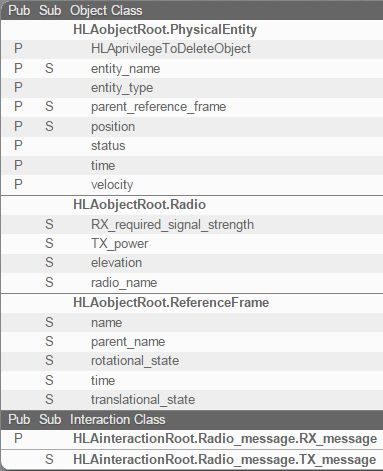
\includegraphics[width=\linewidth]{interactions.png}
		\caption{MWSU Satellite publish/subscribe listing.}
	\label{interactions}
\end{figure}
		
		The FOM (see Figure \ref{fom}) contains descriptions of the Objects, Interactions, and Data Types that federates will use in a federation. Because of this all federates must agree on which FOMs to use. This is arguably the most important part of the HLA standard; it ensures that the designers of each federate communicate in order to come to an agreement on not just the FOM, but on other aspects such as the overall goal of the simulation.
\begin{figure}[!htbp]
	\centering
		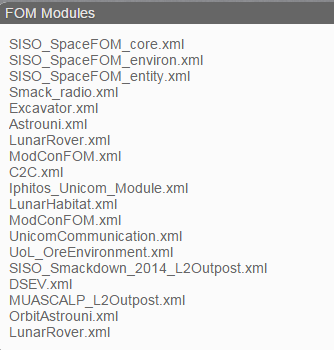
\includegraphics[width=\linewidth]{fom.png}
		\caption{FOMs used in SEE 2016.}
	\label{fom}
\end{figure}		
		
The recommended representation for a federation is called a "lollipop" diagram (see Figure \ref{lollipop}). 
\begin{figure}[!htbp]
	\centering
		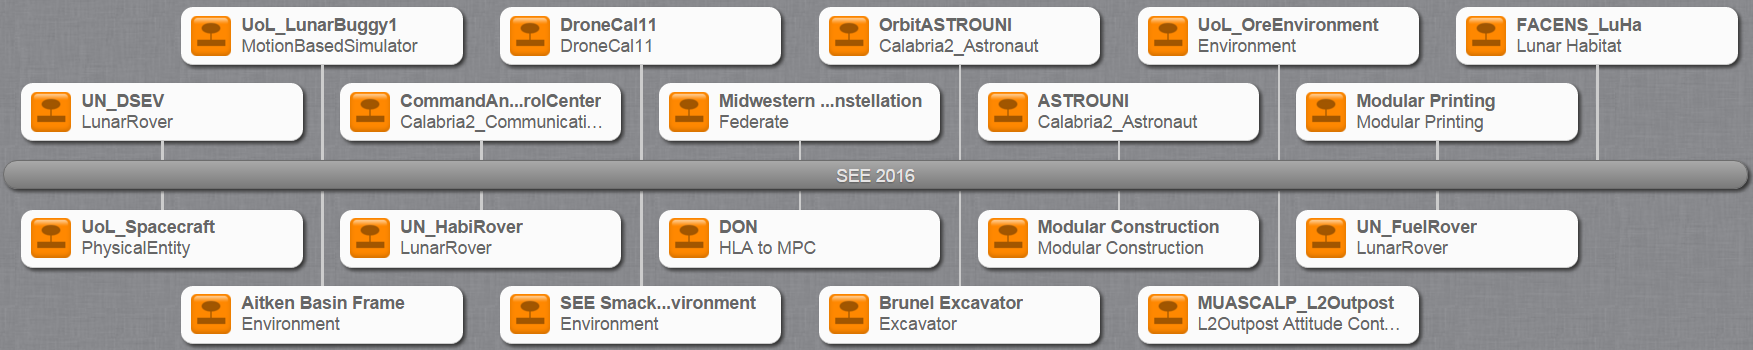
\includegraphics[width=\linewidth]{lollipop.png}
		\caption{SEE 2016 participants lollipop diagram.}
	\label{lollipop}
\end{figure}		
\section{2016 SEE Experience}
The Simulation Exploration Experience, hosted by NASA was an exciting and immersive experience in modeling and distributed simulation.  The 2016 MWSU Sim team consisted of four computer science students, one graduate and three undergraduates, and our sponsoring professor and local HLA expert, Dr. Wei.  We began meeting formally late in the Fall 2015 semester in preparation for our participation in the SEE 2016 workshop at the 2016 SCS Spring Simulation Multi-Conference (SpringSim '16) that took place in Liverpool, England.  This experience allowed us to implement knowledge learned in multiple courses, such as software engineering, discrete system simulation, and contemporary programming.

Our first step in preparing ourselves for writing our own federate was to download the HLA tutorial available on the Pitch website\cite{HLA}.  Once we fully understood the HLA model, we were able to access and complete numerous tutorials on creating federates available to participating SEE team members in the SEE Assembla repository. The following subsections describe the MWSU Sim team satellite federate, and the team's experiences interacting with industry professions, NASA engineers, and college students from around the world.

\subsection{Satellite Constellation \& Lunar Visualization Module}
The Satellite Constellation \& Lunar Visualization module first propagates and then renders satellite constellations. STK\rq{}s numerical propagator is invoked to generate the orbits of different satellites. The constellation is achieved by STK\rq{}s High Precision Orbit Propagator (HPOP) which is a part of the Orbit Propagation Library (OPL). By numerically integrating the various forces affecting satellites, HPOP brings high fidelity orbit propagation into our MWSU communication satellites.

When the whole federation is running on Pitch RTI, a 6-satellite constellation is designed over Aitken Basin to maximize the time each satellite is in view of the surface entities as shown in Figure \ref{Satellites}.
\begin{figure}[!htbp]
	\centering
		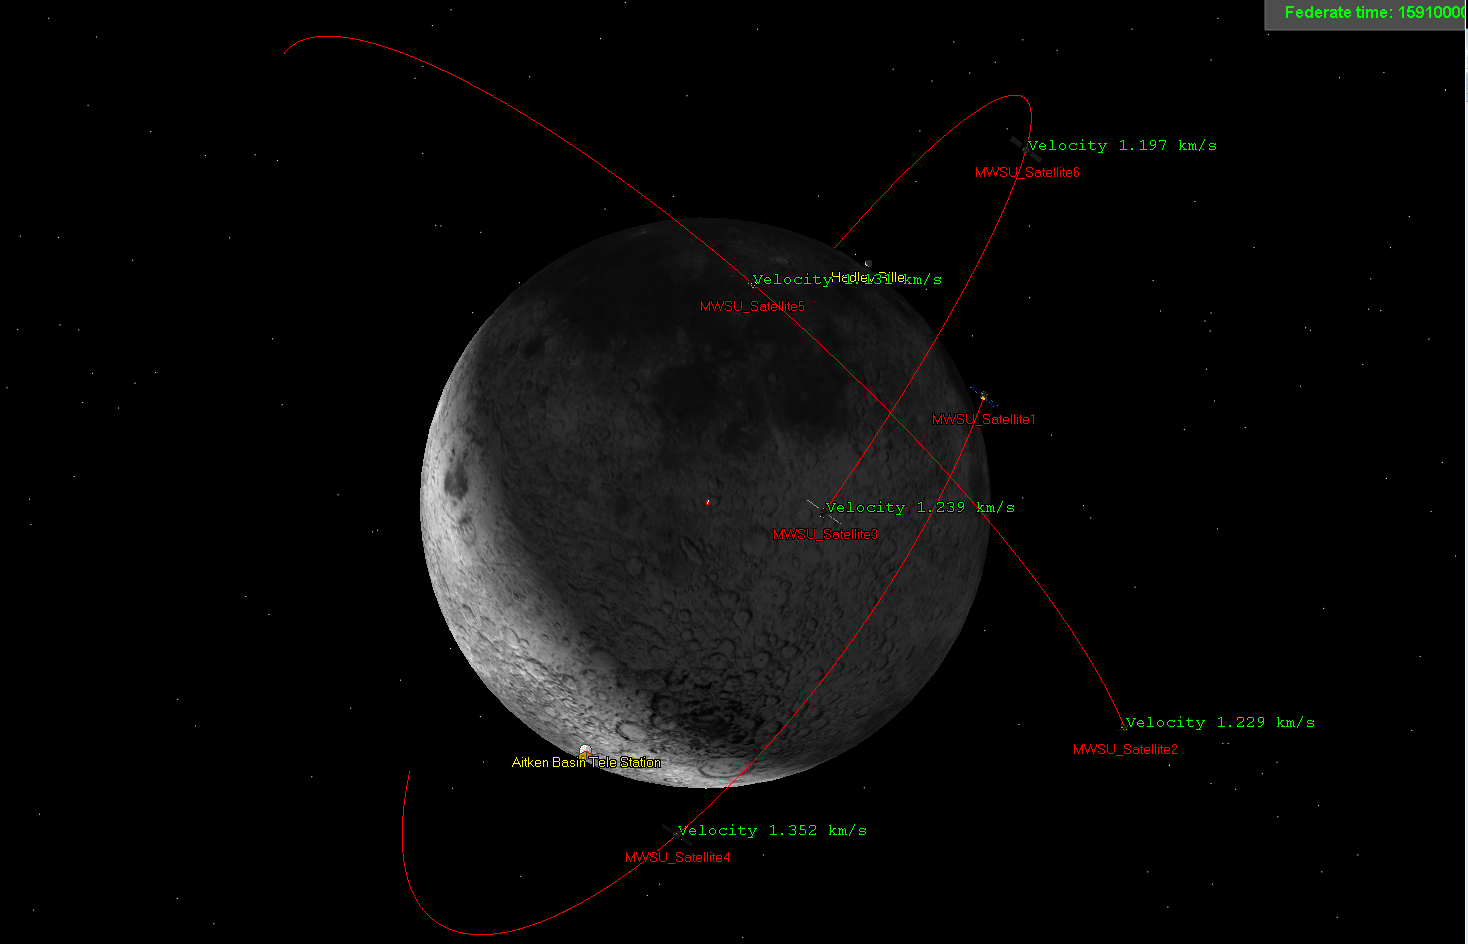
\includegraphics[width=\linewidth]{Satellites.PNG}
		\caption{MWSU communication satellites federate.}
	\label{Satellites}
\end{figure}

The architecture of the Satellite Constellation \& Lunar Visualization module is shown in, Figure \ref {Class}, a UML class diagram.
\begin{figure}[!htbp]
	\centering
		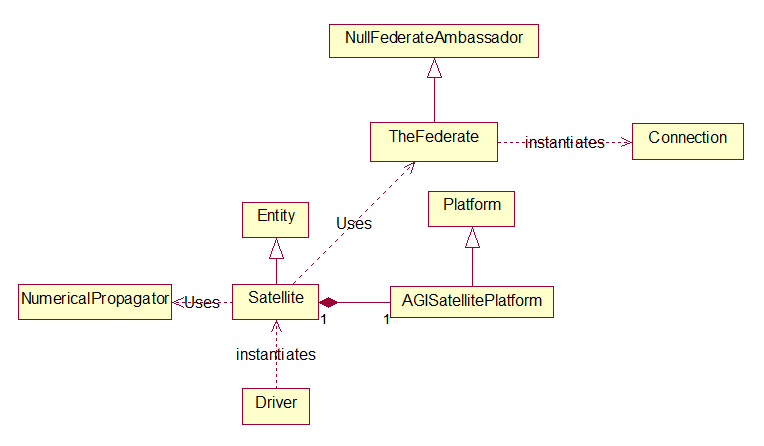
\includegraphics[width=\linewidth]{ClassDiagram.png}
		\caption{MWSU satellite constellation \& lunar visualization module class diagram.}
	\label{Class}
\end{figure}
 
In this module, \uml{Satellite} is a subclass of the \uml{PhysicalEntity} object class defined in the SISO\_SpaceFOM\_entity FOM.  Once the MWSU federate was granted time advance by the NASA time regulating federate, each satellite published its logical time, entity name, reference frame and most up-to-date Cartesian coordinate position. Other federates which were interested in obtaining the attributes of satellites could subscribe to and receive the updates sent by the MWSU federate.

Regarding the propagation of orbits, each satellite uses a numerical propagator provided by STK to propagate its orbit. STK Components increases the fidelity and accuracy of its simulation of orbits by providing a variety of environment and force models. In our case, spherical harmonic gravity of the moon and solar radiation force are considered during the propagation of a satellite\rq{}s orbit. The gravity model of the moon is read in from LunarGravityField\_LP100K.grv file. It is then used to construct the immutable field by selecting the desired fidelity degree and order of the represented field, as well as configuring other options such as the inclusion of tidal data. This field is then used to define the force at a given position. Those force models together with the six orbital elements are the parameters required to uniquely identify a specific orbit: semi major axis, eccentricity, inclination, argument of perigee, right ascension of the ascending node (RAAN) and true anomaly. These parameters were used to propagate the position, orientation, and other attributes of the satellites over time using the numerical propagator which we found to provide accurate orbits. 

In our effort to visualize satellites and their orbits in STK\rq{}s Insight3D viewer, we adopted the STK Components\rq{} \uml{Platform} type which can be used to model satellites, facilities, aircraft, and other ``real-world\rq\rq{} objects. Simply put, an \uml{AGISatellitePlatform} object is created for each \uml{Satellite} object which stores: the name of the satellite, a time-varying position and orientation calculated by the numerical propagator. By adding the \uml{AGISatellitePlatform} into the Insight3D viewer, the visualization of satellites was accomplished.

\subsection{\textit{Tag Ups} \& SpringSim '16}
Starting in November 2015, the MWSU Sim team participated in weekly \textit{tag ups} which occurred at 09:00 CST (06:00 UTC) every Wednesday.  These hour-long meetings utilized a software called VSEE, a visual telecommunication software, that allowed teams from universities around the world, representatives from Pitch and VT M{\"A}K, as well as NASA engineers at both Johnson Space Center(JSC) and Kennedy Space Center(KSC) to communicate and share their progress.  As March 2016 approached, the VSEE \textit{tag ups} were used for preliminary connection testing. During these testing \textit{tag ups}, the Pitch RTI was initiated, then the three NASA world origination federates were connected to the RTI.  Once the simulated world had been instantiated, each team was asked individually to attempt to connect their federate to the Pitch RTI.  Connection of the MWSU satellite federate to the Pitch RTI was performed by first connecting to the VPN, initializing our satellite federate, and upon request from the VSEE meeting organizer, connection to the Pitch RTI.  

The MWSU Sim team participated remotely, via VSEE, that took place at the 2016 SCS Spring Simulation Multi-Conference (SpringSim '16) in Liverpool, England.  During SEE 2016, a lunar mission was simulated. NASA JSC, KSC and 12 universities from three continents participated in this year\rq{}s distributed simulation event. All participants conformed to the IEEE HLA standard 1516-2010 for modeling and simulation. As usual, NASA provided basic support to the entire simulation mission, JSC regulated the time of the simulation while KSC provided real-time visualization of the simulation mission. Each university contributed to the lunar simulation by implementing a part of the entire simulation called a federate (More HLA terminologies are available in \cite{HLA}). A description of the SEE 2016 simulated mission follows: Astronauts explore a huge impact crater close to the south pole of the moon, called Aitken Basin.  Viewers are then introduced to a number of new lunar research units and construction sites: a 3D-printing site by University of Alberta (Canada), a supply depot, oxidizer and propellant production facility by University of Bordeaux (France), an astronaut habitat site by Facens (Brazil), a cargo rover by Florida Institute of Technology, a fuel rover by University of Nebraska, a lunar buggy and an unmanned aerial vehicle (UAV) by University of Liverpool (England).

The peaceful exploration operation is suddenly interrupted by the detection of an incoming asteroid by an asteroid detection system developed by University of Genoa (Italy). The command and communication center \cite{falcone2014simulation} developed by University of Calabria (Italy) alerts all physical entities on the surface of the moon, and the communication satellites developed by Midwestern State University alert the lunar buggy which is out of reach of the command and control center.

During the simulation, all nineteen federates connected successfully to the runtime infrastructure (RTI) provided by Pitch Technologies and were able to advance time (see Figure \ref{lollipop}). Each rectangle represents a joined federate and the middle gray bar denotes the RTI.

\section{Lessons Learned}
During the integration test and the final demo, we found several problems with our federate.  The MWSU federate was able to locate all physical entities in the Insight3D viewer, and verify the location and motion information of different entities in the orbit of the moon or on the surface.  

However, several problems with our federate were found during the integration testing:

Problem 1: Significant time required to populate six satellites.
Solution: This problem is understandable, as the STK numerical propagator calculates a large amount of data for each satellite in order to achieve high fidelity rendering.  By using background calculation capabilities, we achieved a reduction in the time required by parallelizing the satellite propagations.

Problem 2: MWSU federate worked well with Pitch RTI but failed to run on M{\"A}K RTI. When testing on M{\"A}K RTI, exception ``unsatisfiedLinkError makRtiJava1516e.dll: the specified procedure could not be found\rq\rq{} is thrown.
Solution: MWSU federate is a Java application built in Eclipse. This is an old problem with M{\"A}K RTI which does not work with the most recent version of the Java IDE. We attempted to downgrade our Java IDE environment/code in order to communicate with the M{\"A}K RTI, as suggested by members of the 2012 UAHuntsville team \cite{bulgatz2012design}. We were unable to solve this problem and have informed engineers at VT M{\"A}K. We hope this issue can be fixed for SEE 2017.

Problem 3: MWSU federate kept throwing NullPointer exceptions due to other teams failing to provide the latest Attribute Handle Value Map or they provided Attribute Handle Value Map that misses certain attribute values.
Solution: It is a good software engineering principle to not expect federates developed by other teams to behave exactly as expected. Proper and robust exception handling mechanisms were added to help solve this problem.

Problem 4: For our Insight3D viewer, entities on the surface of the moon and those orbiting the moon were represented through markers and text. Since there were so many entities in 2016, the text and markers tended to bloat the viewer and hinder its readability.
Solution: A distance constraint on the visibility of the marker was added so that a marker would only become visible when the distance between the camera and the entity was less than 1000km. If the moon was viewed at a great distance, only the text representing the name of the entity could be seen in the Insight3D viewer.

Problem 5: During testing, we found that some HLA callbacks were never called when they were supposed to be called.
Solution: HLA provides different versions of the same callback, for instance, there are three reflectAttributeValues callbacks. Since the specific callback version the RTI would invoke could not be predicted with optimal success, we added all three callback versions defined in \uml{TheFederate} class and placed the same implementation code in three reflectAttributeValues() functions with different signatures.
 
Problem 6: When a federate resigned from the federation, the Insight3D viewer still kept the marker and text representing the physical entity of that resigned federate.
Solution: Added code to clear the marker and text when the callback method removeObjectInstance was called.

Problem 7: Synchronization exception occurred during the demonstration in insight3DTimeChanged() method of class \uml{LCANSatManager} due to different threads competing on the otherEntitiesToBeDrawn list. This caused the Insight3D viewer to crash.
Solution: Our current solution, although not optimal due to time constraints, was to surround the trouble code with a try-catch block in order to prevent the entire Insight3D viewer from crashing during the event. A better solution would be to add a mutual exclusion lock on this resource. The future team should be aware that this problem has not been solved properly.

\section{Future Team Participation}
The more teams that participate in SEE, the better the experience for everyone involved.  If you would like to start a SEE Sim team at your university please visit the http://www.exploresim.com/team.\\
The requirements to start a team are:
\begin{enumerate}
	\item Minimum team must have at least one college faculty advisor and one student with knowledge of C++ and/or JAVA with the readiness to learn HLA 	 		Evolved, use standards and participate in an inter-university internationl simulation experience.  
	\item Teams can consist of a class, independent researchers, a departmental project, an interdepartmental project or inter-university undertaking.
	\item each team should have a team leader responsible for communication with the SEE Operations, Technical and Executive leaders and committees.
\end{enumerate}

The steps to start a team of your own are as follows:
\begin{enumerate}
	\item Read the requirements necessary to form a team (mentioned above).
	\item Fill out and submit teh team official interest form.
	\item Wait to be contacted by SEE General Manager Stephen Paglialonga.
\end{enumerate}

% conference papers do not normally have an appendix

% trigger a \newpage just before the given reference
% number - used to balance the columns on the last page
% adjust value as needed - may need to be readjusted if
% the document is modified later
%\IEEEtriggeratref{8}
% The "triggered" command can be changed if desired:
%\IEEEtriggercmd{\enlargethispage{-5in}}

% references section

% can use a bibliography generated by BibTeX as a .bbl file
% BibTeX documentation can be easily obtained at:
% http://www.ctan.org/tex-archive/biblio/bibtex/contrib/doc/
% The IEEEtran BibTeX style support page is at:
% http://www.michaelshell.org/tex/ieeetran/bibtex/
\bibliographystyle{IEEEtran}
\bibliography{bibliography}
% argument is your BibTeX string definitions and bibliography database(s)
%\bibliography{IEEEabrv,../bib/paper}
%
% <OR> manually copy in the resultant .bbl file
% set second argument of \begin to the number of references
% (used to reserve space for the reference number labels box)

%\begin{thebibliography}{1}

%\bibitem{IEEEhowto:kopka}
%H.~Kopka and P.~W. Daly, \emph{A Guide to \LaTeX}, 3rd~ed.\hskip 1em plus
%  0.5em minus 0.4em\relax Harlow, England: Addison-Wesley, 1999.

%\end{thebibliography}




% that's all folks
\end{document}
